\begin{figure}
  \setlength{\unitlength}{\textwidth}
  \begin{picture}(1,0.3)(0,0.8)
    % % %90
    \put(0.025,0.83){\includegraphics[width=0.5\unitlength]{../FnP/gnuplot/vel_time_history_60_0.075.eps}}
    \put(0.495,0.83){\includegraphics[width=0.5\unitlength]{../FnP/gnuplot/vel_time_history_165_0.175.eps}}
    
    \put(0.02,0.95){ $\displaystyle\frac{V}{D}$} 	
    % \put(0.56,1.02){ $\frac{V}{D}$}
 	
    \put(0.25,0.80){ $\displaystyle\frac{tU}{D}$} 	
    \put(0.73,0.80){ $\displaystyle\frac{tU}{D}$}

    \put(0.095,1.035){(a)}
    \put(0.565,1.035){(b)}

  \end{picture}

  \caption{Time histories of velocity at two different $\zeta$ and $U^*$ which produce the same mean power ($1.2\times10^{-3}$). Data presented in (a) are at $\ustar=60$, $\zeta=0.075$ and (b) are at $\ustar=165$, $\zeta=0.175$. Both data sets were obtained using Quasi-steady state assumption using input $C_y$ parameters at $Re=165$. Shedding is evident in both signals as a high frequency fluctuation but the amplitude of the slower fluctuations remains constant in both cases. \JL{KASUN: The different scale on the x-axes make these two plots difficult to compare. I think a more powerful comparison can be made by keeping the x-scale the same (include more periods of the case at $U^*=60$). Then it is clear that even though the oscillation happens over a longer time, the average power output is constant. You could also include a plot where you rescale time by the time scale I derived, $\tau=\tau=t(a_1/m^*)(U/D)$. I'm pretty certain that, apart from the high frequency shedding component, the two plots would lok the same using this time scale}}
    \label{fig:time_hostory_velocity_same_power}
\end{figure}

 